\section{Triangle Inequality Computations}
To determine if the triangle inequality has failed, one must look to determine if the difference matrix, $|A|+|B|-|A+B|$, and determine that it not positive semi-definite which is verified by its eigenvalues,
or checking the determinant of the diagonal minors. Let us first consider an example where the failure of the triangle inequality occurs.

\begin{example}
Consider: 
$$
A = \begin{bmatrix}
    -1 & 1 \\
    -1 & 1
\end{bmatrix} \quad
\text{and} \quad
I_2 = \begin{bmatrix}
    1 & 0 \\
    0 & 1
\end{bmatrix}
$$
We wish to verify that: $|A+I_2| \leq |A|+|I_2|$ is not true. It is noted that $\sqrt{I_2}=I_2$. Using Theorem \ref{theorem1} allows simple computation of the matrix absolute value for matrix $A+I_2$ and matrix $A$.
\begin{align*}
    |A+I_2| &= 
    \left|\begin{bmatrix}
        -1 & 1 \\
        -1 & 1
    \end{bmatrix} 
    +
    \begin{bmatrix}
        1 & 0 \\
        0 & 1
    \end{bmatrix}\right| 
    = 
    \left|\begin{bmatrix}
        0 & 1 \\
        -1 & 2
    \end{bmatrix}\right| \\
    &=
    \left(
    \begin{bmatrix}
        0 & -1 \\
        1 & 2
    \end{bmatrix}
    \begin{bmatrix}
       0 & 1 \\
        -1 & 2 
    \end{bmatrix}\right)^\frac{1}{2} 
    =
    \begin{bmatrix}
        1 & -2 \\
        -2 & 5
    \end{bmatrix}^\frac{1}{2}\\
    &= 
    \frac{1}{\sqrt{8}}
    \begin{bmatrix}
        2 & -2\\
        -2 & 6
    \end{bmatrix}\\
    &=
    \begin{bmatrix}
         \frac{\sqrt{2}}{2} & \frac{-\sqrt{2}}{2} \\
        \frac{-\sqrt{2}}{2} & \frac{3\sqrt{2}}{2}
    \end{bmatrix}
\end{align*}
Similarly, 
\begin{align*}
    |A| &= \left|
    \begin{bmatrix}
        -1 & 1\\
        -1 & 1
    \end{bmatrix} \right|\\
    &=
    \left(
    \begin{bmatrix}
        -1 & -1\\
        1 & 1
    \end{bmatrix}
    \begin{bmatrix}
        -1 & 1\\
        -1 & 1
    \end{bmatrix}\right)^\frac{1}{2} 
    = 
    \begin{bmatrix}
        2 & -2 \\
        -2 & 2
    \end{bmatrix}^\frac{1}{2}\\
    &= 
    \frac{1}{2}
    \begin{bmatrix}
        2 & -2\\
        -2 & 2
    \end{bmatrix}\\
    &=
    \begin{bmatrix}
        1 & -1\\
        -1 & 1
    \end{bmatrix}
\end{align*}
If we apply the triangle inequality with these three matrices found, we get the following result:
\begin{align*}
    |A+I_2| &\leq |A| +I_2 \\
    \implies\begin{bmatrix}
        \frac{\sqrt{2}}{2} & \frac{-\sqrt{2}}{2} \\
        \frac{-\sqrt{2}}{2} & \frac{3\sqrt{2}}{2}
    \end{bmatrix}
    &\leq
    \begin{bmatrix}
        1 & -1 \\
        -1 & 1
    \end{bmatrix}
    +
    \begin{bmatrix}
        1 & 0 \\
        0 & 1
    \end{bmatrix}\\
    \Leftrightarrow 
    \begin{bmatrix}
        0 & 0 \\
        0 & 0
    \end{bmatrix}
    &\leq
    \begin{bmatrix}
        2 &-1\\
        -1 & 2
    \end{bmatrix} 
    -
    \begin{bmatrix}
        \frac{\sqrt{2}}{2} & \frac{-\sqrt{2}}{2} \\
        \frac{-\sqrt{2}}{2} & \frac{3\sqrt{2}}{2}
    \end{bmatrix}\\
    \implies
    \begin{bmatrix}
        0 & 0 \\
        0 & 0
    \end{bmatrix}
    &\leq
    \begin{bmatrix}
        2 - \frac{\sqrt{2}}{2} & -1 + \frac{\sqrt{2}}{2}\\
        -1 + \frac{\sqrt{2}}{2} & 2 - \frac{3\sqrt{2}}{2}
    \end{bmatrix} 
\end{align*}
If the difference matrix $|A|+I_2-|A+I_2|$ is not positive semidefinite then the triangle inequality would have failed.
We will check the determinants of the minor diagonals for this difference matrix to determine this.
\begin{align*}
    \left|2-\frac{\sqrt{2}}{2}\right| &\approx 2 - 0.707 \\
    & = 1.23 > 0
    \text{, and}\\
    \begin{vmatrix}
         2 - \frac{\sqrt{2}}{2} & -1 + \frac{\sqrt{2}}{2}\\
        -1 + \frac{\sqrt{2}}{2} & 2 - \frac{3\sqrt{2}}{2}
    \end{vmatrix}
    &= \left( 2 - \frac{\sqrt{2}}{2}\right)\left(2 - \frac{3\sqrt{2}}{2}\right) - \left(-1 + \frac{\sqrt{2}}{2}\right)^2\\
    &= \left(4 - 3\sqrt{2} - \sqrt{2} + \frac{3}{2} - \left(1 - \sqrt{2} + \frac{1}{2}\right)\right)\\
    &= 4 - 3\sqrt{2}\\
    &\approx 4 - 4.243\\
    &= -0.234 < 0.
\end{align*}
This shows that the difference matrix is not PSD; consequently, the triangle inequality fails given the choice of $A$ and $I_2$.
\end{example}
\subsection[methods]{Computational Methods}

The Triangle Inequality of the matrix absolute value was investigated using Python. Four key tasks were implemented into their own function for this paper.

\begin{enumerate}
    \item Verifying a Triangle Inequality
    \item Computing the Matrix Absolute Value of any Matrix, $A \in M_n$
    \item Verifying the Positivity of Any Matrix, $A \in M_n$
    \item Computing a random matrix in $M_n$ of varying entry types and varying entry ranges
\end{enumerate}
The complete python project can be found in the Github repository referenced in this paper. In this appendix we provide the pseudocode for each key function, without the usage of helper functions that would be found in the full project.

\paragraph{\textbf{(i) Implementing a Test for the Triangle Inequality}} The procedure of testing the triangle inequality could have simply been included in our statistics scripts, but we wanted the flexibility of being able to test different functions as lengths, as well as changing the notion of positivity if deemed necessary.

\begin{algorithm}
    \caption{Check Triangle Inequality, \texttt{triangle\_inequality()}}
    \begin{algorithmic}[1]
        \REQUIRE{Two elements, $A$, $B$ $\in V$,}
        \REQUIRE{A function to act as length, $d: V \rightarrow W$}
        \REQUIRE{A function to act as positivity, $positive: W \rightarrow \texttt{bool}$}
        \STATE Compute lengths $d(A)$, $d(B)$, $d(A+B)$
        \STATE difference = $d(A) + d(B)-d(A+B)$
        \IF{$positive(\text{difference})==\texttt{true}$}
        \STATE \textbf{return} True
        \ELSE
        \STATE \textbf{return} False
        \ENDIF
    \end{algorithmic}
\end{algorithm}

\paragraph{\textbf{(ii) Implementing the Matrix Absolute Value}} We defined a python function for the matrix absolute value, which would serve as our length function in our triangle inequality function. The absolute value of a matrix was implemented in two ways, where the first implementation determines the square root of $A^*A$ using the Spectral Decomposition. This way is the fastest as it exploits the fact that $A^*A$ is always diagonalizable. The second implementation uses a SciPy function, \texttt{absm}, to determine the square root using the Schur Decomposition. This is the most numerically stable way of computing the square root of any matrix regardless of whether it is diagonalizable \cite{Edvin}.

\begin{algorithm}
    \caption{Compute Matrix Absolute Value (Spectral), \texttt{matrix\_absolute\_value()}}
    \begin{algorithmic}[1]
        \REQUIRE{Single matrix, $A \in M_n$,}
        \STATE{Compute $A^*A$}
        \STATE{Compute $P$, $D$ of the spectral decomposition $A^*A = PDP^*$}
        \STATE{Compute $D^\frac{1}{2}$ by taking the square root each element of $D$}
        \STATE{Compute $|A| = PD^\frac{1}{2}P^*$}
        \STATE{\textbf{return} $|A|$}
    \end{algorithmic}
\end{algorithm}

\paragraph{\textbf{(ii) Implementing a test for Matrix Positivity}} The matrix positivity was implemented in two different ways. The first implementation of determining if a matrix is positive semi-definite, solves for all the eigenvalues, and asserts than the minimum eigenvalue is greater than or equal to zero.
\begin{algorithm}
    \caption{Check Matrix Positivity (Eigenvalues), \texttt{matrix\_positivity()}}
    \begin{algorithmic}[1]
        \REQUIRE{Single matrix, $A \in M_n$,}
        \REQUIRE{Tolerance, \texttt{tol},}
        \STATE{Compute $\sigma(A)$, the set of all eigenvalues of $A$}
        \STATE{Determine $\lambda_{\min} = \min(\sigma(A))$}
        \IF{$\lambda_{\min} >$ -\texttt{tol}}
        \STATE{\textbf{return} True}
        \ELSE{}
        \STATE{\textbf{return} False}
        \ENDIF{}
    \end{algorithmic}
\end{algorithm}
The second implementation for matrices in $M_2$ asserts that the trace is greater than zero and the determinant is greater than or equal to zero, recalling that for any matrix $A$, $\text{tr} A = \sum_{i}^{n} \lambda_i$, and $\text{det} A = \prod_{i}^{n} \lambda_i$. \begin{algorithm}
    \caption{Check Matrix Positivity of $M_2$ (Trace and Determinant), \texttt{matrix\_positivity()}}
    \begin{algorithmic}[1]
        \REQUIRE{Single matrix, $A \in M_2$,}
        \REQUIRE{Tolerance, \texttt{tol},}
        \STATE{Compute $\text{tr}A = A[0,0] + A[1,1]$, the Trace of $A$}
        \STATE{Compute $\text{det}A = (A[0,0] \times A[1,1]) - (A[0,1] \times A[1,0])$, the Determinant of $A$}
        \IF{$|\text{tr}A| < \texttt{tol}$ \AND$|\text{det}A| < \texttt{tol}$}
        \STATE{\textbf{return} True}
        \ELSIF{$\text{tr}A > \texttt{tol}$ \AND$\text{det}A > \texttt{tol}$}
        \STATE{\textbf{return} True}
        \ELSE{}
        \STATE{\textbf{return} False}
        \ENDIF{}
    \end{algorithmic}
\end{algorithm}
Each implementation, requires a tolerance to determine if the minimum eigenvalue (or trace/determinant) was approximately zero. If the minimum eigenvalue is minuscule, then checking the determinant might be less likely to be near our tolerance as it is the product of all eigenvalues. If all the eigenvalues are fractional, then directly checking the minimum eigenvalue will be less likely to be near our tolerance. Alternating between different implementations of determining PSD and of the matrix absolute value were useful in demonstrating that our results were not sensitive to differences in numerical stability and reproducible through different approaches.
\subsection{Results}

The percentage of Triangle Inequality failures was investigated for matrix pairs, $A, B \in M_n$ with varying entry types and dimension. For real ($M_n(\mathbb R)$) or integer ($M_n(\mathbb Z)$) type entries, the values range from $(-k, k)$, $k\in \mathbb Z$. For Gaussian integer ($M_n(\mathbb Z[i])$) or complex ($M_n(\mathbb C)$) type entries, the values are of the form $a+bi$, where $a,b$ range from $(-k, k)$, $k\in \mathbb Z$. Sample failure percentages for each entry types were calculated from 100,000 randomly chosen pairs within a fixed entry range $(-k, k)$. True failure percentages were also calculated for pairs $A, B \in M_2(\mathbb Z)$ by exhaustively determining all possible pairs (with replacement) with entry ranges $(-k, k)$, $k \geq 7 \in \mathbb Z$. (\autoref{fig:sample_true_fail_rates_n2_varied_types_ranges})
\begin{figure}[H]
    \centering
    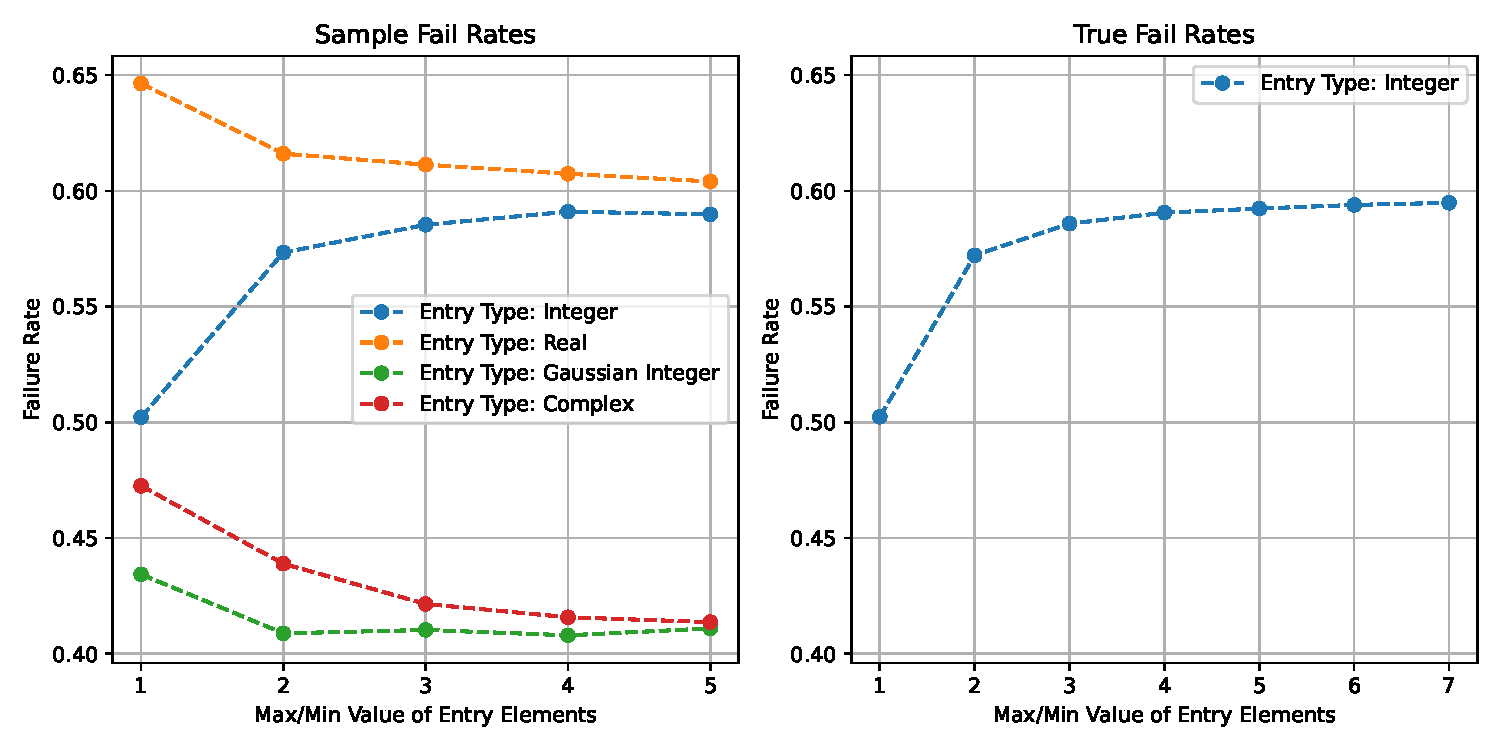
\includegraphics[width=\textwidth]{assets/sample_true_fail_rates_n2_varied_types_ranges.pdf}
    \caption{Comparison of sample and true triangle inequality failure rates of $M_2$. Each sample point contains 100,000 randomly chosen matrix pairs, with standard tolerance}\label{fig:sample_true_fail_rates_n2_varied_types_ranges}
\end{figure}

The effect of increasing the dimensions of the matrix pairs were also investigated. Sample Failure Rates for all entry types at a standard tolerance of $10^{-7}$ were produced for $2\leq n\leq 5$. (\autoref{fig:sample_fail_rate_varied_n_type_range})

\begin{figure}[H]
    \centering
    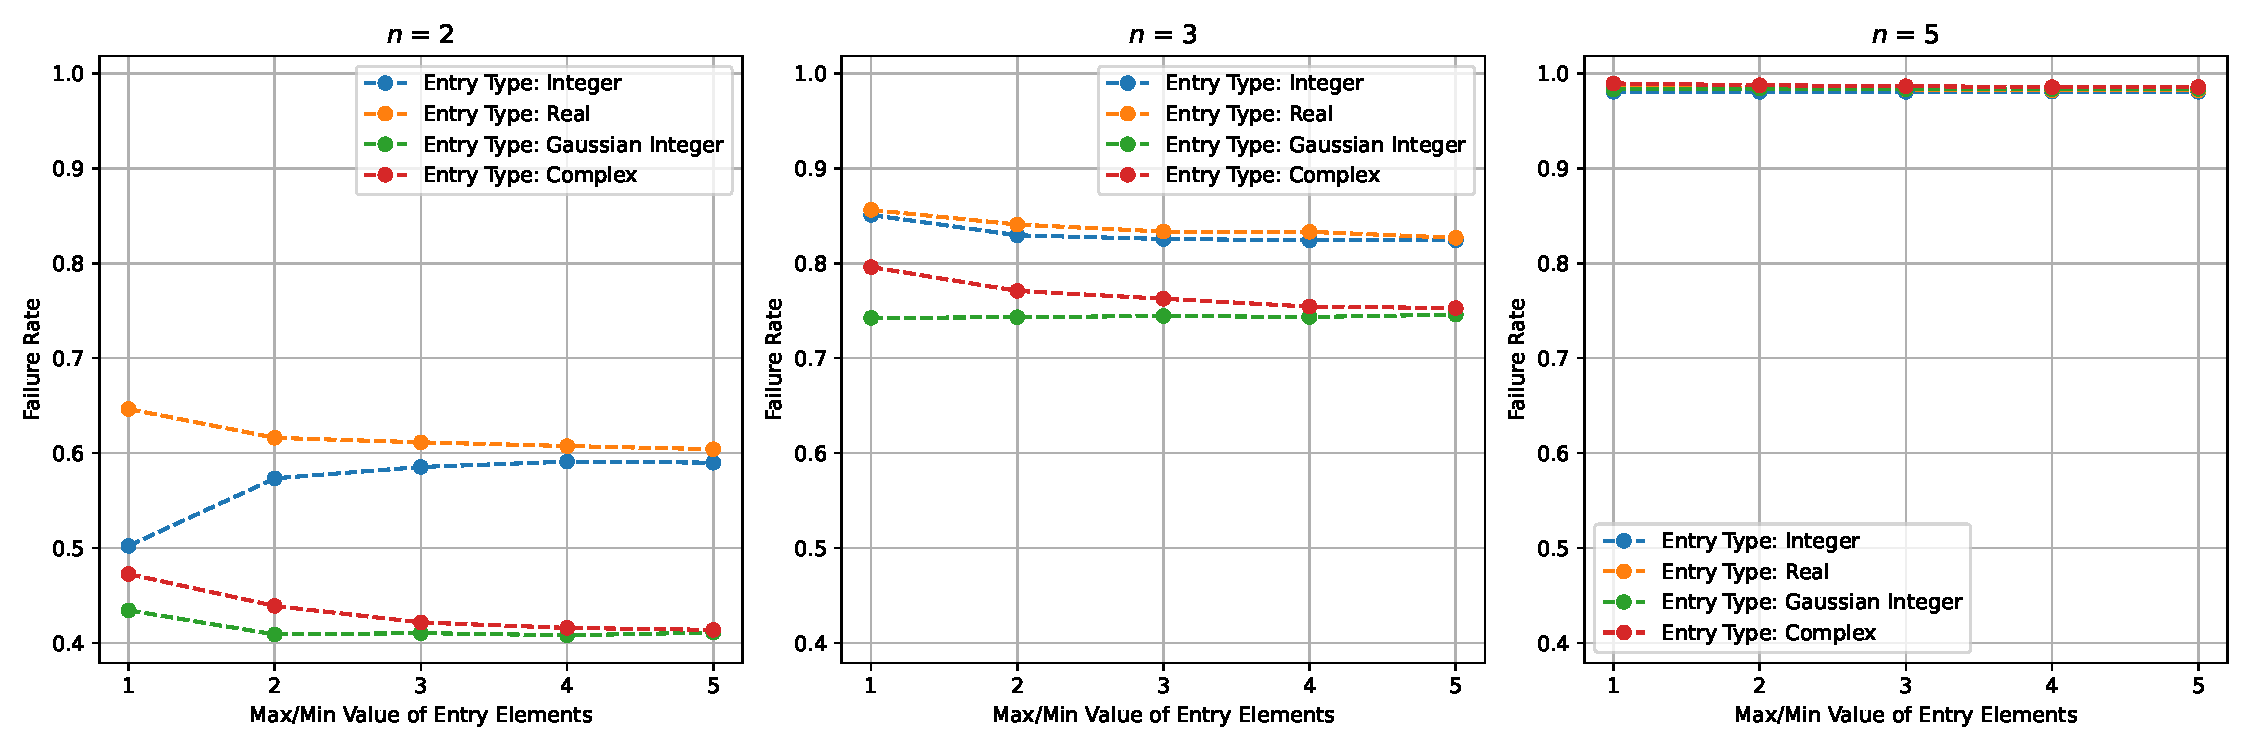
\includegraphics[width=\textwidth]{./assets/sample_fail_rate_varied_n_type_range.pdf}
    \caption{Changes in fail rate as $n$ increases. Each sample point contains 100,000 randomly chosen matrix pairs, with standard tolerance}\label{fig:sample_fail_rate_varied_n_type_range}
\end{figure}